\documentclass{article}

% Document extensibility %
%
% Disables native paragraph indentation
\usepackage{parskip} 
%
% Provides further bullet options for lists
\usepackage{enumitem}

% Mathematical symbol and statement packages %
%
% Necessary
\usepackage{amsmath}
\usepackage{amssymb}
%
% Extensive fraction notation
\usepackage{xfrac}
%
% Generic mathematical commands
% Notable: \degree, \celcius
\usepackage{gensymb}
%
% Variable vector notation (arrow above variable)
\usepackage{esvect}
%
% Multiline boxed equations
\usepackage{empheq}

% Graphic packages %
%
% Diagrams and illustrations
\usepackage{tikz}
\usetikzlibrary{positioning}
%
% Image insertion
\usepackage{graphicx}

% Document content %
%
% Change title of table of contents
\renewcommand{\contentsname}{Units and Vectors}

\title{Homework 1}
\author{Corey Mostero}
\date{Student ID: 256652}

\begin{document}

% Command `\hr` to insert horizontal rules
\newcommand{\hr}{\par\noindent\rule{\textwidth}{0.4pt}}

\maketitle
\newpage

\tableofcontents

\section{Book}

\subsection{1.21}

\begin{tikzpicture}
    \draw[very thick, ->] (0, 0) -- (0, 10) node [above] { $+\hat{y}$ };
    \draw[very thick, ->] (0, 0) -- (10 ,0) node [right] { $+\hat{x}$ };
    \fill (0, 0) circle [radius=2pt] node [above right] { ($0$km,$0$km) };

    \draw[thick, ->, blue] (0, 0) node [left] { Start - $A$ } -- (0, 2.6) node [midway, above, sloped] { $2.6$km } -- (0, 2.6) node [above] { $B$ };
    \draw[thick, ->, blue] (0, 2.6) -- ++(0:4) node [midway, above] { $4.0$km };
    \draw[thick, blue, fill=blue] (4.0, 2.6) -- ++(0:0) node [above] {$C$} -- ++(45:3.1) node [midway, above, sloped] { $3.1$km } -- ++(0:0) circle [radius=2pt] node [above] { End - $D$ };
    \draw[dashed, black] (4.0, 2.6) -- ++(0:2) node [above, midway] { $\theta = 45\degree$ };
\end{tikzpicture}

Variables:
\begin{align*}
    \vv{AB} & = \left((0)\hat{x} + (2.6)\hat{y}\right)\text{km} \\
    \vv{BC} & = \left((4.0)\hat{x} + (0)\hat{y}\right)\text{km} \\
    \vv{CD} & = 3.1\text{km} \\
    \theta & = 45\degree \\
    \vv{CD}_x & = ? \\
    \vv{CD}_y & = ? \\
    \vv{AD} & = ?
\end{align*}
Finding components of $ \vv{CD} $:
\begin{align*}
    \cos(\theta) & = \frac{\vv{CD}_x}{\text{hyp.}} \\
    \vv{CD}_x & = \text{hyp.} \cdot \cos(\theta) \\
              & = 3.1\text{km} \cdot \cos(45\degree) \\
              & = 2.2\text{km} \\
    \sin(\theta) & = \frac{\vv{CD}_y}{\text{hyp.}} \\
    \vv{CD}_y & = \text{hyp.} \cdot \sin(\theta) \\
              & = 3.1\text{km} \cdot \sin(45\degree) \\
              & = 2.2\text{km}
\end{align*}
$$ \vv{CD} = \left((2.2)\hat{i} + (2.2)\hat{j}\right)\text{km} $$
Finding the vector $ \vv{AD} $:
\begin{align*}
    \vv{AD} & = \vv{AB} + \vv{BC} + \vv{CD} \\
            & = \left(\vv{AB}_x + \vv{BC}_x + \vv{CD}_x\right)\hat{i} + \left(\vv{AB}_y + \vv{BC}_y + \vv{CD}_y\right)\hat{j} \\
            & = \left(0\hat{i} + 4.0\hat{i} + 2.2\hat{i}\right)\text{km} + \left(2.6\hat{j} + 0\hat{j} + 2.2\hat{j}\right)\text{km} \\
            & = \left(6.6\hat{i} + 4.8\hat{j}\right)\text{km}
\end{align*}
Finding magnitude of $ \vv{AD} $:
\begin{align*}
    \|\vv{AD}\| & = \sqrt{(AD_x)^2 + (AD_y)^2} \\
                & = \sqrt{(6.6\text{km})^2 + (4.8\text{km})^2} \\
                & = 8.16\text{km}
\end{align*}
Finding direction of $ \vv{AD} $:
\begin{align*}
    \tan(\theta) & = \frac{\text{opp.}}{\text{adj.}} \\
    \theta & = \arctan\left(\frac{\text{opp.}}{\text{adj.}}\right) \\
           & = \arctan\left(\frac{4.8\text{km}}{2.2\text{km}}\right) \\
           & = 65.38\degree \text{ N of E}
\end{align*}
Solution:
\begin{empheq}[box=\fbox]{align*}
    & \text{Magnitude: } 8.16\text{km} \\
    & \text{Direction: } 65.38\degree \text{ N of E}
\end{empheq}

\section{Lab Manual}

\subsection{172}

\begin{enumerate}[label=\alph*)]
    \item Prove that $ \vv{A} \cdot \vv{B} = \vv{B} \cdot \vv{A} $
    \item Show that $ \vv{A} \cdot \vv{B} $ can be interpreted either as $ B $ times the component of $ \vv{A} $ in the direction of $ \vv{B} $, or as $ A $ times the component of $ \vv{B} $ in the direction of $ \vv{A} $.
    \item Calculate the dot product of the two vectors, $ \vv{A} \cdot \vv{B} $, given below: (No units)
        \begin{enumerate}[label=\arabic*)]
            \item $ \vv{A} = 20 $ along the +X axis, $ \vv{B} = 15 $ at $ 37\degree $ above the +X axis.
            \item $ \vv{A} = 6 $ at $ 20\degree $ above the +X axis, $ \vv{B} = 10 $ at $ 70\degree $ above the +X axis.
            \item $ \vv{A} = 3 $ along the +X axis, $ \vv{B} = 4 $ along the +X axis.
            \item $ \vv{A} = 4 $ along the +X axis, $ \vv{B} = 4 $ along the -X axis.
            \item $ \vv{A} = 0.3 $ along the +X axis, $ \vv{B} = 0.5 $ at $ 135\degree $ to $ \vv{A} $
            \item $ \vv{A} = 12 $ along the +X axis, $ \vv{B} = 7 $ along the +Y axis.
        \end{enumerate}
\end{enumerate}

a)
\begin{align*}
    \vv{A} \cdot \vv{B} & = \vv{B} \cdot \vv{A} \\
    \vv{A}_x\vv{B}_x + \vv{A}_y\vv{B}_y & = \vv{B}_x\vv{A}_x + \vv{B}_y\vv{A}_y
\end{align*}
Which can be rewritten as
\begin{equation*}
    \boxed{
        \vv{A}_x\vv{B}_x + \vv{A}_y\vv{B}_y = \vv{A}_x\vv{B}_x + \vv{A}_y\vv{B}_y
    }
\end{equation*}

b) \\
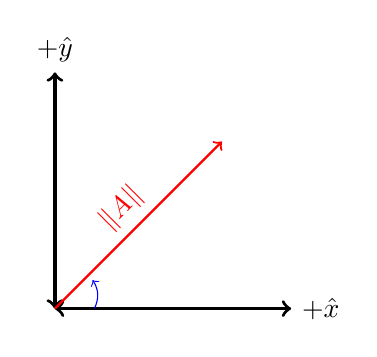
\begin{tikzpicture}
    \draw[very thick, <->] (0,0) -- (0,3) node [above] { $+\hat{y}$ };
    \draw[very thick, <->] (0,0) -- (3,0) node [right] { $+\hat{x}$ };
    \draw[thick, ->, red] (0,0) -- (45:3) node [midway, above, sloped] { $\|\vv{A}\|$ };

    \draw[transparent] (0,0) -- (45:0.5) [above] node (theta) {};
    \path[blue, bend right, ->] (0.5,0) edge (theta); 
\end{tikzpicture}

Begin by finding the component of $ \vv{A} $ in the direction of $ \vv{B} $
\begin{align*}
\end{align*}

\subsection{173 (b)}

\subsection{174}

\subsection{184}

\end{document}
